\documentclass[border={7pt 0pt 70pt 0pt},varwidth]{standalone}
\usepackage{amsmath}
\usepackage[dvipsnames]{xcolor}%colors
\usepackage{tikz-cd,tikz-3dplot} 
\usepackage{diagbox}
\usepackage{makecell}
\usepackage{adjustbox}
\usepackage{multirow}
\usepackage[width=0.5,tiewidth=0.7]{strands}
\usepackage{array}

\newcommand{\fakestar}{*}
\begin{document}
\begin{table}[]
\arraycolsep=1pt
\[
 \setcellgapes{0ex}\makegapedcells
\begin{array}{ccccccc}

    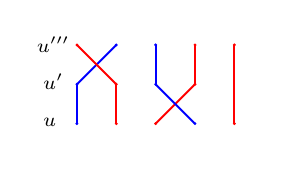
\begin{tikzpicture}[baseline=(current bounding box)]
    \node at (-0.3,0.06) {$\scriptstyle u\phantom{'}$};
    \node at (2.3,0.06) {$\phantom{\scriptstyle u'}$};
    \node at (-0.3,0.53) {$\scriptstyle u'$};
    \node at (-0.3,1) {$\scriptstyle u'''$};
    \node at (1.5,-0.15) {$\phantom{\scriptstyle i+1}$};
    \tie[color=blue,bull=1,bulletie=0.01,style=solid]{{2,1},{1,0.5},{1,0}}
    \tie[color=red,bull=1,bulletie=0.01,style=solid]{{1,1},{2,0.5},{2,0}}
    \tie[color=red,bull=1,bulletie=0.01,style=solid]{{4,1},{4,0.5},{3,0}}
    \tie[color=blue,bull=1,bulletie=0.01,style=solid]{{3,1},{3,0.5},{4,0}}
    \tie[color=red,bull=1,bulletie=0.01,style=solid]{{5,1},{5,0}} 
    \end{tikzpicture}        &=&
    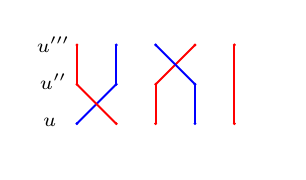
\begin{tikzpicture}[baseline=(current bounding box)]
        \node at (-0.3,0.06) {$\scriptstyle u\phantom{'}$};
        \node at (2.3,0.06) {$\phantom{\scriptstyle u'}$};
        \node at (-0.3,0.53) {$\scriptstyle u''$};
        \node at (-0.3,1) {$\scriptstyle u'''$};
        \node at (1.5,-0.15) {$\phantom{\scriptstyle i+1}$};
        \tie[color=blue,bull=1,bulletie=0.01,style=solid]{{2,1},{2,0.5},{1,0}}
        \tie[color=red,bull=1,bulletie=0.01,style=solid]{{1,1},{1,0.5},{2,0}}
        \tie[color=red,bull=1,bulletie=0.01,style=solid]{{4,1},{3,0.5},{3,0}}
        \tie[color=blue,bull=1,bulletie=0.01,style=solid]{{3,1},{4,0.5},{4,0}}
        \tie[color=red,bull=1,bulletie=0.01,style=solid]{{5,1},{5,0}} 
        \end{tikzpicture}
        &\hspace{10mm}$\,$
        &
    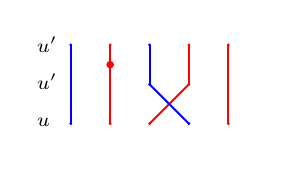
\begin{tikzpicture}[baseline=(current bounding box)]
    \node at (-0.3,0.06) {$\scriptstyle u\phantom{'}$};
    \node at (2.3,0.06) {$\phantom{\scriptstyle u'}$};
    \node at (-0.3,0.53) {$\scriptstyle u'$};
    \node at (-0.3,1) {$\scriptstyle u'$};
    \node at (1.5,-0.15) {$\phantom{\scriptstyle i+1}$};
    \tie[color=blue,bull=1,bulletie=0.01,style=solid]{{1,1},{1,0}}
    \tie[color=red,bull=1,bulletie=0.01,style=solid]{{2,1},{2,0}}
    \tie[color=red,bull=1,bulletie=0.01,style=solid]{{4,1},{4,0.5},{3,0}}
    \tie[color=blue,bull=1,bulletie=0.01,style=solid]{{3,1},{3,0.5},{4,0}}
    \tie[color=red,bull=1,bulletie=0.01,style=solid]{{5,1},{5,0}} 
    \tie{{2,0.75}}
    \end{tikzpicture}        &=&
    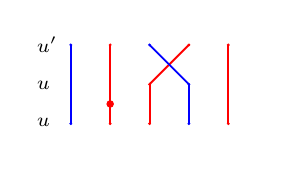
\begin{tikzpicture}[baseline=(current bounding box)]
        \node at (-0.3,0.06) {$\scriptstyle u\phantom{'}$};
        \node at (2.3,0.06) {$\phantom{\scriptstyle u'}$};
        \node at (-0.3,0.53) {$\scriptstyle u\phantom{'}$};
        \node at (-0.3,1) {$\scriptstyle u'$};
        \node at (1.5,-0.15) {$\phantom{\scriptstyle i+1}$};
        \tie[color=blue,bull=1,bulletie=0.01,style=solid]{{1,1},{1,0}}
        \tie[color=red,bull=1,bulletie=0.01,style=solid]{{2,1},{2,0}}
        \tie[color=red,bull=1,bulletie=0.01,style=solid]{{4,1},{3,0.5},{3,0}}
        \tie[color=blue,bull=1,bulletie=0.01,style=solid]{{3,1},{4,0.5},{4,0}}
        \tie[color=red,bull=1,bulletie=0.01,style=solid]{{5,1},{5,0}} 
        \tie{{2,0.25}}
        \end{tikzpicture}
           \\
D_3^{u,u'} \fakestar D_1^{u',u'''} &=& D_1^{u,u''} \fakestar D_3^{u'',u'''}&& D_3^{u,u'}\fakestar e_2^{u'}   &=& e_2^{u} \fakestar D_3^{u,u'}
\end{array}
\]
\end{table}
\end{document}